\chapterimage{orange2.jpg}
\chapterspaceabove{6.75cm} 
\chapterspacebelow{7.25cm} 
\chapter{Random Variable and Discrete Distribution}
Random variables are fundamental concepts in probability theory, describing 
quantities whose values result from random phenomena. This chapter delves into 
discrete random variables and their distributions, exploring how they are used to modeling 
and analyze situations where outcomes are countable.

\begin{itemize}
    \item \textbf{Definition of Random Variables:} We start by defining random 
    variables and discussing their basic properties, including how they function 
    within the framework of probability theory.
    
    \item \textbf{Expectation and Variance:} This section covers the computation 
    and implications of expectation and variance, which describe the average 
    outcome of a random variable and the spread of its outcomes, respectively.
    
    \item \textbf{Common Discrete Distributions:} We explore well-known 
    distributions such as the Binomial and Poisson distributions, which are 
    essential for modeling many real-world processes.
    
    \item \textbf{Other Discrete Distributions:} Additional discrete distributions 
    are discussed, providing insights into more specialized or less commonly 
    encountered models.
    
    \item \textbf{Properties of Random Variables, PDF, and CDF:} The chapter 
    concludes with an examination of the mathematical properties of random 
    variables, including their probability distribution functions and cumulative 
    distribution functions.
\end{itemize}

Each section includes exercises that challenge the reader to apply theoretical 
concepts to practical problems, reinforcing learning and enhancing understanding 
of random variables and discrete distributions.

\section{Random Variable}
We First define random variables and discuss their basic properties, including how they function within the framework of probability theory.
In a short word, a random variable is a functional relation between the possible outcomes of a random experiment
and the probability of each outcome. It assigns a real number to each outcome in the sample space of a random experiment.
\begin{definition}[Random Variable]
    A \textbf{random variable} is a function \( X: S \rightarrow \mathbb{R} \) 
    where \( S \) is the sample space of a random experiment. This function 
    assigns a real number to each outcome in the sample space \( S \). 
    
    The mapping \( X \) is defined such that for any outcome \( \omega \) 
    in the sample space \( S \), \( X(\omega) \) specifies a real number 
    that represents a possible value of the random variable in the context 
    of the experiment. This allows the random variable to quantify 
    the outcomes of the experiment in numerical terms.
\end{definition}

A random variable \( X \) can be thought of as a rule or a function that assigns 
a specific number to each possible outcome of a random experiment. The sample 
space \( S \) includes all possible outcomes of this experiment. For each 
outcome \( \omega \) in \( S \), the random variable \( X \) gives a number 
\( X(\omega) \). This number is not random; it is fixed for each outcome 
\( \omega \).

This mapping can be a little abstract, but in a short word, random variable is a way to represent 
the outcomes of a random experiment in numerical terms, which make it easier to analyze and make predictions about the outcomes of the experiment.

Here are some practical examples of random variables.
\begin{example}[Tossing a Coin]
    Consider a random experiment where we toss a fair coin. Define the sample space 
    \( S = \{\text{Heads}, \text{Tails}\} \). Let \( X \) be a random variable that 
    assigns \( 1 \) if the outcome is Heads and \( 0 \) if the outcome is Tails. Thus, 
    \( X(\text{Heads}) = 1 \) and \( X(\text{Tails}) = 0 \). Here, \( X \) is used to 
    numerically represent the outcomes of a coin toss.
    \end{example}
    
    \begin{example}[Daily Temperature]
    Consider measuring the high temperature in a particular city on a given day. 
    Define \( X \) to be the random variable representing the high temperature 
    recorded on that day. If the thermometer reads 20 degrees Celsius, then 
    \( X(\omega) = 20 \) where \( \omega \) is the outcome of that day's temperature 
    measurement. This example shows how random variables can be used to model 
    quantitative data in environmental studies.
    \end{example}
    
    \begin{example}[Number of Customers]
    Suppose a shop wants to analyze the number of customers that enter the store 
    each day. Let \( X \) be a random variable representing the total number of 
    customers on any given day. If 250 customers enter the shop on a particular day, 
    then \( X(\omega) = 250 \), indicating the count of customers as the outcome 
    of the random variable.
    \end{example}
    
    \begin{example}[Sum of Dice Rolls]
    Consider rolling two six-sided dice and let \( X \) be the random variable 
    representing the sum of the numbers on the two dice. The sample space \( S \) 
    consists of all pairs of numbers from 1 to 6 for each die. For an outcome 
    \( \omega = (3, 4) \), where the first die shows 3 and the second die shows 4, 
    the random variable \( X \) would give \( X(\omega) = 3 + 4 = 7 \). This is a 
    classical example used in probability theory to introduce the concept of sum 
    distributions.
    \end{example}

The purpose of this mapping is to numerically represent the results of 
random processes, allowing us to apply mathematical tools to analyze 
and make predictions about these processes. The mapping defined by \( X \) 
is deterministic within the experiment context—once the outcome \( \omega \) 
is realized, the value \( X(\omega) \) is definitively known. 

Another question is that, are random variable always discrete? The answer is no. Random variables can be either discrete or continuous, depending on the nature of the outcomes they represent. Discrete random variables are those that take on a finite or countably infinite number of distinct values, while continuous random variables can take on any value within a specified range. In this chapter, we focus on discrete random variables and their distributions, 
which are essential for modeling and analyzing situations where outcomes are countable.
We have seen many examples of discrete random variables in the previous examples. 
And this chapter involves indeed only discrete random variables. Still, we provide an example of continuous random variables for completeness.

\begin{example}[Height of Students]
Let \( X \) be a continuous random variable representing the height (in centimeters) 
of students in a high school. The exact height of a student can be any value within 
a range, making \( X \) a continuous random variable. The probability of \( X \) 
taking any specific value is zero, but probabilities can be assigned to ranges of 
values (e.g., the probability that a student's height is between 160 cm and 170 cm).
\end{example}

\begin{example}[Time Required to Complete a Task]
Suppose \( T \) represents the time (in hours) required to complete a specific task. 
\( T \) is a continuous random variable because the completion time can be any 
real number within a certain interval, depending on various factors like speed, 
efficiency, and interruptions.
\end{example}

\begin{example}[Amount of Rainfall]
Let \( R \) be a continuous random variable representing the amount of rainfall 
(in millimeters) received in a city on a given day. Rainfall can be measured as 
any non-negative real number, making \( R \) a perfect example of a continuous 
random variable, where you can find the probability of receiving more than a 
certain amount of rainfall but not the probability of an exact amount.
\end{example}

\begin{example}[Temperature Measurement]
Consider \( \Theta \) as a continuous random variable representing the temperature 
(in degrees Celsius) at noon in a particular location. Temperature is inherently 
continuous as it can take any value within a possible range, and minor variations 
are always possible, making \( \Theta \) continuously variable.
\end{example}

You may have realized that dealing with continuous random variables requires knowledge of calculus and integration.
In this chapter, we focus on discrete random variables, which are easier to work with and provide a solid foundation for understanding more complex probability concepts.
\subsection{Analysis of Random Variables}
The random variable itself seems to be a simple concept, but it is essential in probability theory.
What can we do with random variables? We can analyze them in various ways to understand the underlying probability distributions and make predictions about the outcomes of random processes.
We have seen many examples of analyzing random events and the probability of events in the previous chapters.
In those cases, we found probability given a specific event or a set of events.
With random variable, we can model the pattern of probability distribution of the outcomes of the random process
in all cases.

Here is a simple example of analyzing a random variable in a given situation.
\begin{example}[Tossing Three Coins]
    Suppose our experiment consists of tossing three fair coins. If we let \( Y \) denote the number of heads that appear, then \( Y \) is a random variable taking on one of the values 0, 1, 2, and 3 with respective probabilities:

\begin{itemize}
    \item \( P(Y = 0) = P(\text{T, T, T}) = \frac{1}{8} \)
    \item \( P(Y = 1) = P(\text{T, T, H}) + P(\text{T, H, T}) + P(\text{H, T, T}) = 3 \times \frac{1}{8} = \frac{3}{8} \)
    \item \( P(Y = 2) = P(\text{T, H, H}) + P(\text{H, T, H}) + P(\text{H, H, T}) = 3 \times \frac{1}{8} = \frac{3}{8} \)
    \item \( P(Y = 3) = P(\text{H, H, H}) = \frac{1}{8} \)
\end{itemize}

Since \( Y \) must take on one of the values 0 through 3, we must have:
\[ 
1 = P\left( \bigcup_{i=0}^{3} \{Y = i\} \right) = \sum_{i=0}^{3} P(Y = i)
\]
which, of course, is in accord with the preceding probabilities, because all these
cases are disjoint and combine to cover all possibilities.
\end{example}

With random variable, we can model more complex situations and analyze the probability distribution of the outcomes.
Here is a more complex example of analyzing a random variable in a given situation.
\begin{example}[Coin Flipping]
    Consider an experiment where we flip a coin that has a probability \( p \) of 
coming up heads. We continue flipping the coin until either a head appears or 
we have flipped the coin \( n \) times. Let \( X \) denote the number of times 
the coin is flipped. Then, \( X \) is a random variable that can take on values 
from 1 to \( n \), where each value corresponds to the number of flips made.

The probabilities for each outcome are calculated as follows:
\begin{itemize}
    \item \( P(X = 1) = p \) (The probability of getting heads on the first flip)
    \item \( P(X = 2) = (1 - p) p \) (The probability of getting tails first, then heads)
    \item \( P(X = 3) = (1 - p)^2 p \) (The probability of getting tails twice, then heads)
    \item \dots
    \item \( P(X = n - 1) = (1 - p)^{n-2} p \) (The probability of getting tails \( n-2 \) times, then heads)
    \item \( P(X = n) = (1 - p)^{n-1} \) (The probability of getting tails \( n-1 \) times, if \( n \) flips are made and no heads appear)
\end{itemize}

As a verification, the sum of all probabilities must equal 1:
\[
\sum_{i=1}^{n} P(X = i) = p \sum_{i=1}^{n-1} (1 - p)^{i-1} + (1 - p)^{n-1}
\]
\[
= p \frac{1 - (1 - p)^{n-1}}{1 - (1 - p)} + (1 - p)^{n-1}
\]
\[
= p \left(\frac{1 - (1 - p)^{n-1}}{p}\right) + (1 - p)^{n-1}
\]
\[
= 1 - (1 - p)^{n-1} + (1 - p)^{n-1}
\]
\[
= 1
\]

This confirms that the calculated probabilities are correct and all possibilities 
have been accounted for.
\end{example}

\subsection{Discrete Random Variables and Discrete Distributions}
Now we shall give a strict definition to distribution of discrete random variables, which we 
also call discrete probability distribution.
\begin{definition}[Discrete Probability Distribution]
    A \textbf{discrete probability distribution} is a function that assigns 
    probabilities to each possible value of a discrete random variable. 
    This function specifies the probability of each possible outcome of the 
    random variable, allowing us to analyze the likelihood of different values 
    occurring.
    A discrete probability distribution is characterized by a probability mass function \( p \) which assigns a probability \( p(x) \) to each possible value \( x \) of the discrete random variable \( X \). The function \( p \) satisfies the following conditions:
\begin{itemize}
    \item \( p(x) \geq 0 \) for all \( x \) in the domain of \( X \),
    \item \( \sum_{x} p(x) = 1 \), where the sum extends over all possible values of \( X \).
\end{itemize}

The distribution is \textit{discrete} because the sum involves a countable number of terms, and the random variable \( X \) takes on countable, typically finite, distinct values.
\end{definition}

Probability distributions are modeled using probability functions. Here we also give 
a strict definition to these functions.

\begin{definition}[Probability Measure of Random Variable]
    The probability that \( X \) takes on a specific value \( x \) from \( \mathbb{R} \) is given by:
    \[ P(X = x) = P(\{\omega \in S \mid X(\omega) = x\}) \]
    This expression evaluates the measure of the set of all outcomes \( \omega \) in \( S \) for which the value of the random variable \( X \) equals \( x \).

\end{definition}
Probability measure is a measure of the likelihood of a specific value of a random variable.
While it is not a probability distribution or function, but just an independent measure 
of the likelihood of a specific value of a random variable.

\begin{definition}[Probability Function of Random Variable]
    For a discrete random variable \( X \) defined on a sample space \( S \), the probability function \( P \) can be described by a mapping:
    \[
    P: \mathcal{P}(S) \to [0, 1]
    \]
    where \( \mathcal{P}(S) \) is the power set of \( S \), representing all possible subsets of \( S \). For each event \( A \subset S \), the probability function is defined as:
    \[
    P(A) = \sum_{\omega \in A} P(\{\omega\})
    \]
    assuming \( P(\{\omega\}) \) specifies the probability of the elementary event \( \{\omega\} \).
    
    In the context of a random variable, the mapping can also be represented specifically for the outcomes of \( X \) as:
    \[
    P_X: \mathbb{R} \to [0, 1]
    \]
    with:
    \[
    P_X(x) = P(X = x) = P(\{\omega \in S \mid X(\omega) = x\})
    \]
    This means the probability that some elements $\omega$ of the sample space $S$, where $\omega$ that satisfies $X(\omega)=x$ by the random variable $X$ to some real number $x$ (in the case of discrete distribution, $x\in \Z$).
    
    This function \( P_X \) gives the probability that \( X \) takes any particular value \( x \).    
\end{definition}

We illustrate with an example of fair dice rolling.
\begin{example}[Rolling a Fair Six-Sided Die]
    Let \( X \) be the random variable representing the outcome of rolling a fair six-sided die. The possible outcomes for \( X \) are 1, 2, 3, 4, 5, and 6. Since the die is fair, the probability of each outcome is equal. Thus, the probability function for \( X \) is given by:
    \[
    P(X = x) = \frac{1}{6}, \text{ for } x = 1, 2, 3, 4, 5, 6
    \]
    and \( P(X = x) = 0 \) for all other values of \( x \). We are not plottig it here for clarity, but doesn't mean the function is not defined for other possible value of $X = x\in \{\Z^+ - \{1, 2, 3, 4, 5, 6\}\}$.

\begin{center}
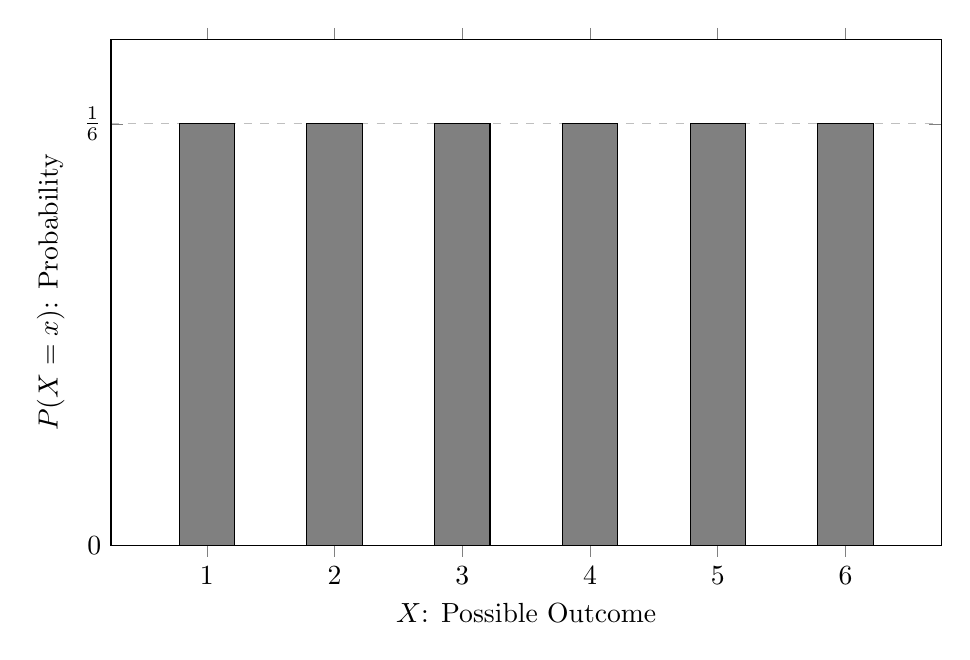
\begin{tikzpicture}
\begin{axis}[
    ybar, 
    bar width=20pt,
    width=\textwidth,
    height=8cm,
    xlabel={$X$: Possible Outcome},
    ylabel={$P(X=x)$: Probability},
    symbolic x coords={1,2,3,4,5,6},
    xtick=data,
    ymin=0, ymax=0.20, % Adjust the maximum y-value appropriately
    ytick={0, 0.1667}, % Use decimal equivalent of 1/6
    yticklabels={0, $\frac{1}{6}$}, % You can still use fractions in labels for clarity
    nodes near coords,
    nodes near coords align={vertical},
    enlarge x limits=0.15,
    ymajorgrids=true,
    grid style=dashed,
]

\addplot[fill=gray, nodes near coords=] coordinates {
    (1,0.1667) (2,0.1667) (3,0.1667) (4,0.1667) (5,0.1667) (6,0.1667)
};
\end{axis}
\end{tikzpicture}
\end{center}

    This plot shows the uniform probability distribution for each outcome of rolling the die.
\end{example}

It is noticeable that for each possible $x$, $P(X=x)$ has the same value $\frac{1}{6}$. 
Actually, this distribution is categorized as a kind of special, but most basic discrete distribution, called \textbf{Uniform Discrete Distribution}.

We have been using the terms discrete distribution and discrete probability function. They are very close to each other, while we need to differentiate them in many aspects.
A probability function and a probability distribution are related but distinct concepts in probability theory. The key difference lies in their scope and representation.

A probability function specifies the probability of each individual outcome or value of a random variable. It provides a point-wise description of the likelihood of different outcomes.

On the other hand, a probability distribution is a more comprehensive concept that encompasses the collective behavior of a random variable. It describes the overall probabilistic properties of the random variable, often by specifying the probabilities associated with different ranges or sets of outcomes.



\subsection{Exercises}

\section{expectation and variance}

\subsection{Exercises}

\section{Common Discrete Distributions}
\subsection{Exercises}

\section{Other Discrete Distributions}
\subsection{Exercises}

\section{Properties of Random Variable, PDF, and CDF}
\subsection{Exercises}



